\section{Ensemble-Methoden}
\label{sec:Ensemble}
\label{sec:wahlklassifizierer}
Die Ensemble-Methoden beschreiben wie verschiedene Entscheidungsbäume trainiert werden, um eine möglichst hohe Diversität zu erzielen. Die Klassifizierungsergebnisse der einzelnen Entscheidungsbäume werden
dann zu einem Ergebnis zusammengefasst \cite{dietterich2002ensemble}.
\newline
\newline
Der \glqq Wahl\grqq-Klassifizierer $H(x) = w_1 h_1(x) + ... + w_K h_K(x)$ fasst eine Menge von Lösungen $\{h_1, ..., h_K\}$ zusammen mit Hilfe einer Menge von Gewichten $\{w_1, ..., w_K\}$, die in der Summe 1
ergeben. Eine Lösung $h_i: D^n \mapsto \setR^m$ weist einer arbiträren, $n$-dimensionalen Menge $D^n$ jeder der $m$ möglichen Klassen eine Wahrscheinlichkeit zu.
Die Summe einer Lösung ist immer 1. Die Klassifizierung einer Lösung ist die Klasse mit der höchsten Wahrscheinlichkeit. Dementsprechend ist analog dazu $H: D^n \mapsto \setR^m$ definiert.
Für gewöhnlich hat jeder Teilnehmer einer Wahl das gleiche Gewicht \cite{dietterich2002ensemble}.
\newline
\newline
\begin{figure}
    \centering
    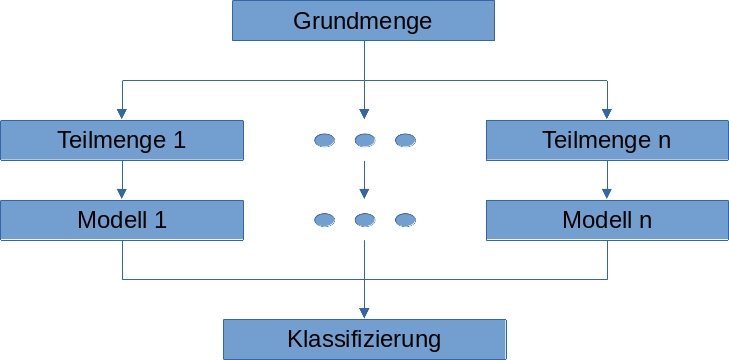
\includegraphics[width=0.6\linewidth]{images/bagging.jpg}
    \caption{Klassifizierungsprozess mit der Bagging-Methode.}
    \label{fig:bagging}
\end{figure}
Bagging ist ein Acronym für \glqq \textbf{B}ootstrap \textbf{agg}regat\textbf{ing}\grqq. Die Idee ist aus einer großen Menge von Trainingsdaten, eine Menge von Mengen von Trainingsdaten zu generieren, folgend mit jedem
dieser Mengen einen Klassifizierer zu trainieren und schließlich alle Klassifizierer, e.g. durch Wählen, zu aggregieren (siehe Abbildung \ref{fig:bagging}) \cite{breiman1996bagging}. Die Methode die dahinter steht nennt
sich \glqq Bootstrap sampling\grqq, welche einen Prozess beschreibt aus einer Grundmenge $m$ mal jeweils $n$ Einträge zu ziehen, die eine Teilmenge bilden \cite{efron1992bootstrap}. Der Name ist folglich aus der Methode
und dem Aggregierungsprozess abgleitet.
\newline
\newline
Random Forest ist eine Erweiterung der Bagging-Methode. Zusätzlich zu der zufällig ausgewählten Menge an Trainingsdaten wird auch zufällig eine Menge von Features ausgewählt. Auf dieser Basis wird ein Menge von
Entscheidungsbäumen generiert die anschließend aggregiert werden \cite{breiman2001random}.
\newline
\newline
Im Vergleich zu Random Forest gehen Extremely Randomized Trees einen Schritt weiter. Anstatt den besten Teilungspunkt zu suchen für die ausgewählten Features, werden zufällig ein Teilungspunkte ausgewählt, aus denen
der beste genutzt wird. Dies soll die Varianz reduzieren. Außerdem wird nicht wie bei der Bagging-Methode auf Teilmengen trainiert sondern auf dem gesamten Set, was den Bias reduzieren soll \cite{geurts2006extremely}.
\newline
\newline
Boosting bezeichnet das Konvertieren eines \glqq schwachen\grqq\ PAC-Algorithmus (\textbf{P}robably \textbf{A}pproximately \textbf{C}orrect), welcher nur leicht besser ist als Raten, in einen \glqq starken\grqq\
PAC-Algorithmus. Ein starker PAC-Algorithmus ist ein Algorithmus der, gegeben $\epsilon, \delta > 0$ und zufällige Beispiele der Trainingsdaten, mit einer Wahrscheinlichkeit $1 - \delta$
klassifiziert mit einem Fehler bis zu $\epsilon$ und die Laufzeit muss polynomial in $\frac{1}{\epsilon}, \frac{1}{\delta}$ und anderen relevanten Parametern sein. Für einen schwachen PAC-Algorithmus gilt das Gleiche
mit dem Unterschied, dass $\epsilon \geq \frac{1}{2} - \gamma$, wobei $\delta > 0$ \cite{freund1997decision}.
\newline
\newline
\begin{figure}
    \centering
    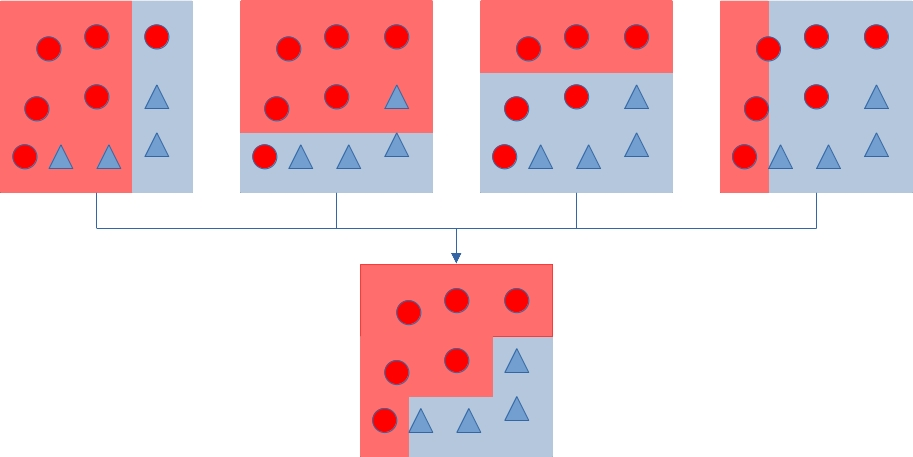
\includegraphics[width=0.6\linewidth]{images/boosting.jpg}
    \caption{Klassifizierungsprozess mit der Boosting-Methode.}
    \label{fig:boosting}
\end{figure}
In Abbildung \ref{fig:boosting} wird illustriert wie drei schwache Lerner jeweils auf eine Teilmenge nacheinander trainiert werden, wobei die Teilmenge des jeweils nächsten von dem Fehler des vorherigen Models abhängt.
Schlussendlich werden alle schwachen Lerner gewichtet aggregiert woraus ein starker Lerner ensteht. In dieser Arbeit wird im speziellen der Boosting Algorithmus \textbf{AdaBoost} von Freund und Schapire verwendet \cite{freund1997decision}.